\section{Requirements}
\label{requirements}
In this chapter, the requirements for the system will be described. Project requirements is a list of the functionality an application must both uphold and support; the criteria on which to judge the application on. As stated earlier, the customer wanted us to explore what possibilities existed for a future Vscan smart device. To not restrict our imagination, the group did not receive a requirements specification from the customer. With the little knowledge we had about the industry at the time, we had to come up with a strategy for how to define these requirements. Exactly how this was done, can be read about in section \ref{workbreakdown}.

\subsection{Business goals}
The main business goal was to improve the usability and effectiveness of the Vscan device. Other goals were to reach out to as large part of the target marked as possible. To realize this, the application had to be easy and fast to use and needed to support integration with legacy systems. This involved being scalable to the extent where the cost of implementing support for a new system was minimal.

\newpage

\subsection{Functional requirements}
The functional requirements describes the concrete functionality the system is required to uphold. Table \ref{funcreqtable} is the full list of functional requirements for the application.


%Tabell for functional requirements
\begin{center}
\tablefirsthead{\hline  \multicolumn{1}{|c}{\tbsp \textbf{FR\#}}
                       & \multicolumn{1}{c}{\textbf{Description}}
                       & \multicolumn{1}{c|}{\textbf{Priority}} \\ \hline\tbsp  }
\tablehead{\hline \multicolumn{3}{|l|}{\small\sl continued from previous page}\\
           \hline \multicolumn{1}{|c}{\tbsp \textbf{FR\#}}
                       & \multicolumn{1}{c}{\textbf{Description}}
                       & \multicolumn{1}{c|}{\textbf{Priority}} \\ \hline\tbsp  }
\tabletail{\hline\multicolumn{3}{|r|}{\small\sl continued on next page}\\\hline}
\tablelasttail{\hline}
\par
\captionof{table}{Functional requirements}

\begin{supertabular}{|p{1cm}|p{9cm}|p{2cm}|}
\label{funcreqtable}

1 & \begin{tabular}[c]{@{}l@{}}
At first startup the application must allow tech-\\
nical personnel to correctly set up the EMR\\
system in use at the current hospital
\end{tabular}  & High \\ \hline

2 & \begin{tabular}[c]{@{}l@{}}
The application must be able to receive images\\
from the Vscan-application
\end{tabular} & High \\ \hline

3 & \begin{tabular}[c]{@{}l@{}}
The application need to allow doctors to authen-\\
ticate with the EMR-system
\end{tabular} & High \\ \hline

4 & \begin{tabular}[c]{@{}l@{}}
The application must be able to identify patients \\
based on SSN
\end{tabular} & High \\ \hline

5 & \begin{tabular}[c]{@{}l@{}}
The application need to be able to upload images \\
to the hospital servers
\end{tabular} & High \\ \hline

\iffalse
2 & \begin{tabular}[c]{@{}l@{}}
The application need to be able to communicate with a interchangeable service over a common interface that\\
is responsible for communication with the EMR itself
\end{tabular} & High \\ \hline
\fi

6 & \begin{tabular}[c]{@{}l@{}}
The application must be able to identify patients \\
based on barcode/QR-code
\end{tabular} & Medium \\ \hline

7 & \begin{tabular}[c]{@{}l@{}}
The application must give feedback to the user\\
on what patient have been identified
\end{tabular} & Medium \\ \hline

8 & \begin{tabular}[c]{@{}l@{}}
The application need to be able to associate ima-\\
ges with the correct patient
\end{tabular} & Medium \\ \hline

9 & \begin{tabular}[c]{@{}l@{}}
The application should let the user view images\\
contained in an examination
\end{tabular} & Medium\\ \hline

10 & \begin{tabular}[c]{@{}l@{}}
The application must not display sensitive infor-\\
mation if the application is in offline mode
\end{tabular} & Medium \\ \hline

11 & \begin{tabular}[c]{@{}l@{}}
An examination must be deleted from the device \\
after being successfully uploaded to the EMR
\end{tabular} & Medium \\ \hline

12 & \begin{tabular}[c]{@{}l@{}}
The application must auto-close and/or auto-log \\
out after a given time of inactivity
\end{tabular} & Medium \\ \hline

13 & \begin{tabular}[c]{@{}l@{}}
The application must be able to be used by more \\
than one user
\end{tabular} & Medium \\ \hline

14 & \begin{tabular}[c]{@{}l@{}}
The application must be able to save the current \\
examination to the database if interrupted before \\
finishing the examination procedure.
\end{tabular} & Medium \\ \hline

15 & \begin{tabular}[c]{@{}l@{}}
The application must be configurable through a \\
settings menu.
\end{tabular} & Medium \\ \hline

16 & \begin{tabular}[c]{@{}l@{}}
The doctor must be able to add comments on \\
associated pictures
\end{tabular} & Low \\ \hline

17 & \begin{tabular}[c]{@{}l@{}}
The doctor must be able to add comments on the \\
examination as a whole
\end{tabular} & Low \\ \hline

18 & \begin{tabular}[c]{@{}l@{}}
The settings view of the application must be pass-\\
word protected
\end{tabular} & Low \\ \hline

19 & \begin{tabular}[c]{@{}l@{}}
The application must support Android version 4 \\
and up
\end{tabular} & Low \\ \hline

\end{supertabular}
\end{center}


\newpage

\subsubsection{Use cases}
This section contains use cases for the high level functional requirements. They are listed both textual and as images to help understand their meaning.

\begin{table}[H]
\renewcommand{\arraystretch}{1.2}
\captionof{table}{Use case: Configuration}
\begin{tabular}{|p{4cm}|p{9cm}|}
\hline
Functional req. ID & 1 \\ \hline
Name & Configuration \\ \hline
Goal & \begin{tabular}[c]{@{}l@{}}
At first startup, the application must allow technical\\
personnel to set up the application to work with the \\
EMR system in use at the current hospital
\end{tabular} \\ \hline
Actors &  Technical user\\ \hline
Start requirements & \begin{tabular}[c]{@{}l@{}}
1.  A preconfigured settings file (XML) must be\\hosted on an available HTTP-server\\
2. The application is deployed to the device
\end{tabular} \\ \hline
End requirements & \begin{tabular}[c]{@{}l@{}}
The application is correctly configured, and is ready\\ for use
\end{tabular} \\ \hline
Main flow & \begin{tabular}[c]{@{}l@{}}
1. User gets prompted to set a technical password\\
2. Writes and repeats password and clicks “OK”\\
3. User gets prompted to input URL to settings file\\
4. Inputs URL to settings file and clicks “Get config”\\
5. Clicks “Confirm”\\
6. User gets prompted to input department username\\/password\\
7. Inputs department username/password and clicks\\ “Confirm”
\end{tabular} \\ \hline
Alternative flow & \begin{tabular}[c]{@{}l@{}}
2a: The technical password (inputed twice) does not\\ match, and the user gets an error message\\
4a: The URL is invalid, and the user gets an error\\ message
\end{tabular} \\ \hline
Parent use case & None \\ \hline
Child use case & 3, 4, 5 \\ \hline
\end{tabular}
\end{table}


\newpage

\begin{figure}[H]
\centering
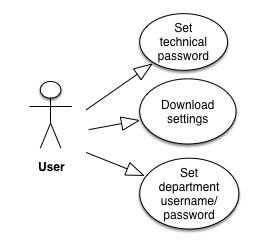
\includegraphics[scale=0.8]{img/usecase/usecase_config1.png}
\caption{Configuration}
\label{fig:config}
\end{figure}

\newpage

\begin{table}[H]
\renewcommand{\arraystretch}{1.2}
\captionof{table}{Use case: Receive images}
\begin{tabular}{|p{4cm}|p{9cm}|}
\hline
Functional req. ID & 2 \\ \hline
Name & Receive images from Vscan \\ \hline
Goal & \begin{tabular}[c]{@{}l@{}}
Receive images from Vscan
\end{tabular} \\ \hline
Actors &  User\\ \hline
Start requirements & \begin{tabular}[c]{@{}l@{}}
1. Vscan provides images ready to be uploaded
\end{tabular} \\ \hline
End requirements & \begin{tabular}[c]{@{}l@{}}
Images are received by the application
\end{tabular} \\ \hline
Main flow & \begin{tabular}[c]{@{}l@{}}
1. The Vscan application triggers the start of the\\ application.
\end{tabular} \\ \hline
Alternative flow & \begin{tabular}[c]{@{}l@{}}
None
\end{tabular} \\ \hline
Parent use case & None \\ \hline
Child use case & None \\ \hline
\end{tabular}
\end{table}



\begin{figure}[H]
\centering
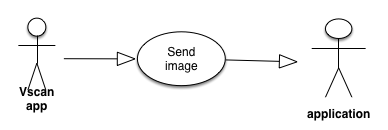
\includegraphics[scale=0.8]{img/usecase/receive.png}
\caption{Receive images from Vscan}
\label{fig:receive_image_uc}
\end{figure}

\newpage

\begin{table}[H]
\renewcommand{\arraystretch}{1.2}
\captionof{table}{Use case: Login}
\begin{tabular}{|p{4cm}|p{9cm}|}
\hline
Functional req. ID & 3 \\ \hline
Name & Login \\ \hline
Goal & \begin{tabular}[c]{@{}l@{}}
To login successfully
\end{tabular} \\ \hline
Actors &  User\\ \hline
Start requirements & \begin{tabular}[c]{@{}l@{}}
1. Login page is displayed\\
2. The user is registered in the system
\end{tabular} \\ \hline
End requirements & \begin{tabular}[c]{@{}l@{}}
The user is successfully logged in
\end{tabular} \\ \hline
Main flow & \begin{tabular}[c]{@{}l@{}}
1. The user gets prompted for username/password\\
2. Inputs username/password and clicks “Login”
\end{tabular} \\ \hline
Alternative flow & \begin{tabular}[c]{@{}l@{}}
2a: Username/password combination is wrong, and\\the
user gets an error message
\end{tabular} \\ \hline
Parent use case & 1 \\ \hline
Child use case & 4, 5 \\ \hline
\end{tabular}
\end{table}


\begin{figure}[H]
\centering
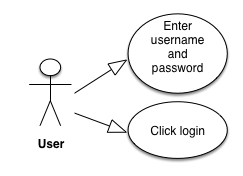
\includegraphics[scale=0.8]{img/usecase/login1.png}
\caption{Login successfully}
\label{fig:login_uc}
\end{figure}

\newpage

\begin{table}[H]
\renewcommand{\arraystretch}{1.2}
\captionof{table}{Use case: Identify}
\begin{tabular}{|p{4cm}|p{9cm}|}
\hline
Functional req. ID & 4 \\ \hline
Name & Identify patient \\ \hline
Goal & \begin{tabular}[c]{@{}l@{}}
Identify patient and retrieve patient data
\end{tabular} \\ \hline
Actors & User\\ \hline
Start requirements & \begin{tabular}[c]{@{}l@{}}
1. Identify patient view is displayed\\
2. User has patients SSN\\
3. Patient exists\\
4. The device has internet connection
\end{tabular} \\ \hline
End requirements & \begin{tabular}[c]{@{}l@{}}
The patient is identified, and patient data is retrieved
\end{tabular} \\ \hline
Main flow & \begin{tabular}[c]{@{}l@{}}
1. User gets prompted to input SSN\\
2. User inputs SSN and clicks “OK”
\end{tabular} \\ \hline
Alternative flow & \begin{tabular}[c]{@{}l@{}}
2a: SSN is invalid, and the user gets an error message\\
\end{tabular} \\ \hline
Parent use case & 1, 3 \\ \hline
Child use case & 4 \\ \hline
\end{tabular}
\end{table}

\begin{figure}[H]
\centering
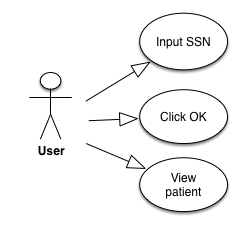
\includegraphics[scale=0.8]{img/usecase/identify1.png}
\caption{Identify patient}
\label{fig:identify_uc}
\end{figure}

\newpage



\begin{table}[H]
\renewcommand{\arraystretch}{1.2}
\captionof{table}{Use case: Upload images}
\begin{tabular}{|p{4cm}|p{9cm}|}
\hline
Functional req. ID & 5 \\ \hline
Name & Upload images to EMR \\ \hline
Goal & \begin{tabular}[c]{@{}l@{}}
Upload examination images to EMR
\end{tabular} \\ \hline
Actors &  User\\ \hline
Start requirements & \begin{tabular}[c]{@{}l@{}}
1. Application is correctly configured\\
2. User is logged in\\
3. Patient has been identified\\
4. Images has been received from Vscan\\
5. The device has internet connection
\end{tabular} \\ \hline
End requirements & \begin{tabular}[c]{@{}l@{}}
Images are uploaded to the EMR server
\end{tabular} \\ \hline
Main flow & \begin{tabular}[c]{@{}l@{}}
1. User is presented with “Review and Upload”-view\\
2. User scrolls down the page, reviewing the \\examination\\
3. User clicks ''Upload'' button\\
4. The application sends all necessary data to the \\service installed \\
5. The service acknowledges that the images were \\uploaded\\
6. The user is redirected to the “Home Screen”-view, \\
and is alerted that the examination was successfully \\uploaded
\end{tabular} \\ \hline
Alternative flow & \begin{tabular}[c]{@{}l@{}}
\textbf{2a)} User wishes to edit the notes before upload,
\\clicks the “Edit”-button, edits the notes and comes\\back to the “Review and Upload”-view \\
\textbf{3a)} User gets prompted with an alert dialog informing \\ that some of the images does not have notes attached\\
\textbf{5a)} Service was not able to upload examination, and \\
the user is returned to the “Home Screen”-view with\\ an alert dialog informing that the upload failed
\end{tabular} \\ \hline
Parent use case & 1, 2, 3, 4 \\ \hline
Child use case & None \\ \hline
\end{tabular}
\end{table}

\begin{figure}[H]
\centering
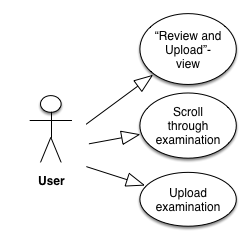
\includegraphics[scale=0.8]{img/usecase/upload1.png}
\caption{Upload images to EMR}
\label{fig:upload_uc}
\end{figure}

\newpage

\subsection{Quality attributes}
The non-functional requirements of a system describes the behavioral functionality required. This section includes a list of the non-functional requirements determined for the project.


\subsubsection{Mobility}
Mobility deals with the problems of movement and affordances of a platform. The scenarios focus on the availability and connectivity issues that might occur when using a mobile device.


\begin{table}[H]
\renewcommand{\arraystretch}{1.2}
\captionof{table}{Quality attributes: Mobility 1}
\begin{tabular}{|p{4cm}|p{9cm}|}
\hline

\textbf{MOB1} & \begin{tabular}[c]{@{}l@{}}
The user should be able to use the application when\\connected to the hospital intranet 
\end{tabular} \\ \hline 

\textbf{Portion of Scenario} & \textbf{Values} \\ \hline
Source of Stimulus & \begin{tabular}[c]{@{}l@{}}
User
\end{tabular} \\ \hline

Stimulus & \begin{tabular}[c]{@{}l@{}} 
Wishes to upload an examination with images and\\comments
\end{tabular} \\ \hline

Artifact & \begin{tabular}[c]{@{}l@{}} 
Smart device
\end{tabular} \\ \hline

Environment & \begin{tabular}[c]{@{}l@{}} 
Runtime with connectivity
\end{tabular} \\ \hline

Response & \begin{tabular}[c]{@{}l@{}} 
Examination successfully uploaded
\end{tabular} \\ \hline

Response Measure & \begin{tabular}[c]{@{}l@{}} 
Max 10 seconds
\end{tabular} \\ \hline

\end{tabular}
\end{table}


%%%%%%%%%%%%%%%	

\begin{table}[H]
\renewcommand{\arraystretch}{1.2}
\captionof{table}{Quality attributes: Mobility 2}
\begin{tabular}{|p{4cm}|p{9cm}|}
\hline

\textbf{MOB2} & \begin{tabular}[c]{@{}l@{}}
The application should manage network loss at any\\stage in its life cycle
\end{tabular} \\ \hline

\textbf{Portion of Scenario} & \textbf{Values} \\ \hline
Source of Stimulus & \begin{tabular}[c]{@{}l@{}}
User
\end{tabular} \\ \hline

Stimulus & \begin{tabular}[c]{@{}l@{}} 
Wishes to upload an examination with images and\\comments
\end{tabular} \\ \hline

Artifact & \begin{tabular}[c]{@{}l@{}} 
Smart device
\end{tabular} \\ \hline

Environment & \begin{tabular}[c]{@{}l@{}} 
Runtime without network connectivity
\end{tabular} \\ \hline

Response & \begin{tabular}[c]{@{}l@{}} 
Offline mode initiated
\end{tabular} \\ \hline

Response Measure & \begin{tabular}[c]{@{}l@{}} 
All examinations are saved locally
\end{tabular} \\ \hline

\end{tabular}
\end{table}


%%%%%%%%%%%%%%%


\subsubsection{Usability}
Usability is concerned with how easy it is for the user to accomplish a desired task. The scenarios focus on ease of use, learning, adaptation and configuration of the system.


\begin{table}[H]
\renewcommand{\arraystretch}{1.2}
\captionof{table}{Quality attributes: Usability 1}
\begin{tabular}{|p{4cm}|p{9cm}|}
\hline

\textbf{USA1} & \begin{tabular}[c]{@{}l@{}}
The application fits into the already existing workflow
\end{tabular} \\ \hline

\textbf{Portion of Scenario} & \textbf{Values} \\ \hline
Source of Stimulus & \begin{tabular}[c]{@{}l@{}}
User
\end{tabular} \\ \hline

Stimulus & \begin{tabular}[c]{@{}l@{}} 
Wishes to incorporate the application in an already\\existing everyday workflow.
\end{tabular} \\ \hline

Artifact & \begin{tabular}[c]{@{}l@{}} 
System
\end{tabular} \\ \hline

Environment & \begin{tabular}[c]{@{}l@{}} 
Normal operation
\end{tabular} \\ \hline

Response & \begin{tabular}[c]{@{}l@{}} 
User understands the workflow
\end{tabular} \\ \hline

Response Measure & \begin{tabular}[c]{@{}l@{}} 
After first complete walk-through user should\\ understand and remember workflow
\end{tabular} \\ \hline
\end{tabular}
\end{table}



%%%%%%%%%%%%%%%



\begin{table}[H]
\renewcommand{\arraystretch}{1.2}
\captionof{table}{Quality attributes: Usability 2}
\begin{tabular}{|p{4cm}|p{9cm}|}
\hline

\textbf{USA2} & \begin{tabular}[c]{@{}l@{}}
It should be easy for the technical user to configure\\ multiple devices
\end{tabular} \\ \hline

\textbf{Portion of Scenario} & \textbf{Values} \\ \hline
Source of Stimulus & \begin{tabular}[c]{@{}l@{}}
Technical User
\end{tabular} \\ \hline

Stimulus & \begin{tabular}[c]{@{}l@{}} 
Wishes to make multiple devices ready to use
\end{tabular} \\ \hline

Artifact & \begin{tabular}[c]{@{}l@{}} 
Vscan probe, smart device and software
\end{tabular} \\ \hline

Environment & \begin{tabular}[c]{@{}l@{}} 
Device not yet set up
\end{tabular} \\ \hline

Response & \begin{tabular}[c]{@{}l@{}} 
Every device is configured in the same way
\end{tabular} \\ \hline

Response Measure & \begin{tabular}[c]{@{}l@{}} 
5-10 minutes for first device, then 2 minutes\\ for the rest
\end{tabular} \\ \hline

\end{tabular}
\end{table}


%%%%%%%%%%%%%%%



\begin{table}[H]
\renewcommand{\arraystretch}{1.2}
\captionof{table}{Quality attributes: Usability 3}
\begin{tabular}{|p{4cm}|p{9cm}|}
\hline

\textbf{USA3} & \begin{tabular}[c]{@{}l@{}}
Minimize the impact of mistakes
\end{tabular} \\ \hline

\textbf{Portion of Scenario} & \textbf{Values} \\ \hline
Source of Stimulus & \begin{tabular}[c]{@{}l@{}}
User
\end{tabular} \\ \hline

Stimulus & \begin{tabular}[c]{@{}l@{}} 
Minimize the impact of errors
\end{tabular} \\ \hline

Artifact & \begin{tabular}[c]{@{}l@{}} 
System
\end{tabular} \\ \hline

Environment & \begin{tabular}[c]{@{}l@{}} 
At runtime
\end{tabular} \\ \hline

Response & \begin{tabular}[c]{@{}l@{}} 
Verify system resources
\end{tabular} \\ \hline

Response Measure & \begin{tabular}[c]{@{}l@{}} 
100\% of examinations should be correct\\when uploaded
\end{tabular} \\ \hline

\end{tabular}
\end{table}


%%%%%%%%%%%%%%%


\begin{table}[H]
\renewcommand{\arraystretch}{1.2}
\captionof{table}{Quality attributes: Usability 4}
\begin{tabular}{|p{4cm}|p{9cm}|}
\hline

\textbf{USA4} & \begin{tabular}[c]{@{}l@{}}
The application should have good\\routine performance
\end{tabular} \\ \hline

\textbf{Portion of Scenario} & \textbf{Values} \\ \hline
Source of Stimulus & \begin{tabular}[c]{@{}l@{}}
User
\end{tabular} \\ \hline

Stimulus & \begin{tabular}[c]{@{}l@{}} 
Wish to navigate to next view
\end{tabular} \\ \hline

Artifact & \begin{tabular}[c]{@{}l@{}} 
System
\end{tabular} \\ \hline

Environment & \begin{tabular}[c]{@{}l@{}} 
At runtime
\end{tabular} \\ \hline

Response & \begin{tabular}[c]{@{}l@{}} 
Next view loaded and is ready for use
\end{tabular} \\ \hline

Response Measure & \begin{tabular}[c]{@{}l@{}} 
Switching views should not take\\more than 0.5 seconds
\end{tabular} \\ \hline

\end{tabular}
\end{table}



%%%%%%%%%%%%%%%


\begin{table}[H]
\renewcommand{\arraystretch}{1.2}
\captionof{table}{Quality attributes: Usability 5}
\begin{tabular}{|p{4cm}|p{9cm}|}
\hline

\textbf{USA5} & \begin{tabular}[c]{@{}l@{}}
The amount of constraints and requirements the\\ 
application put on the environment and its users\\
should be kept to a minimum
\end{tabular} \\ \hline

\textbf{Portion of Scenario} & \textbf{Values} \\ \hline
Source of Stimulus & \begin{tabular}[c]{@{}l@{}}
Application developer
\end{tabular} \\ \hline

Stimulus & \begin{tabular}[c]{@{}l@{}} 
Introduce device and software in workflow
\end{tabular} \\ \hline

Artifact & \begin{tabular}[c]{@{}l@{}} 
System design
\end{tabular} \\ \hline

Environment & \begin{tabular}[c]{@{}l@{}} 
At design time
\end{tabular} \\ \hline

Response & \begin{tabular}[c]{@{}l@{}} 
Users can use the application with or without the \\need for any additional credentials or training
\end{tabular} \\ \hline

Response Measure & \begin{tabular}[c]{@{}l@{}} 
The application depends on the hospitals existing \\technology
\end{tabular} \\ \hline

\end{tabular}
\end{table}

\newpage


%%%%%%%%%%%%%%%


\subsubsection{Security}
Security is a measure of the system's ability to protect data and information from unauthorized access while still providing access to people and systems that are authorized. The scenarios focuses mainly on storage and encryption. 

\begin{table}[H]
\renewcommand{\arraystretch}{1.2}
\captionof{table}{Quality attributes: Security 1}
\begin{tabular}{|p{4cm}|p{9cm}|}
\hline

\textbf{SEC1} & \begin{tabular}[c]{@{}l@{}}
All stored data should be encrypted using industry\\ standards
\end{tabular} \\ \hline

\textbf{Portion of Scenario} & \textbf{Values} \\ \hline
Source of Stimulus & \begin{tabular}[c]{@{}l@{}}
Person
\end{tabular} \\ \hline

Stimulus & \begin{tabular}[c]{@{}l@{}} 
Tries to read database file
\end{tabular} \\ \hline

Artifact & \begin{tabular}[c]{@{}l@{}} 
Data saved by the application
\end{tabular} \\ \hline

Environment & \begin{tabular}[c]{@{}l@{}} 
Under normal operations
\end{tabular} \\ \hline

Response & \begin{tabular}[c]{@{}l@{}} 
File is unreadable
\end{tabular} \\ \hline

Response Measure & \begin{tabular}[c]{@{}l@{}} 
No files should be decrypted without right key
\end{tabular} \\ \hline

\end{tabular}
\end{table}


%%%%%%%%%%%%%%%



\begin{table}[H]
\renewcommand{\arraystretch}{1.2}
\captionof{table}{Quality attributes: Security 2}
\begin{tabular}{|p{4cm}|p{9cm}|}
\hline

\textbf{SEC2} & \begin{tabular}[c]{@{}l@{}}
Data should not be able to leave the application.
\end{tabular} \\ \hline

\textbf{Portion of Scenario} & \textbf{Values} \\ \hline
Source of Stimulus & \begin{tabular}[c]{@{}l@{}}
User
\end{tabular} \\ \hline

Stimulus & \begin{tabular}[c]{@{}l@{}} 
Data being saved outside of database
\end{tabular} \\ \hline

Artifact & \begin{tabular}[c]{@{}l@{}} 
Data within the application
\end{tabular} \\ \hline

Environment & \begin{tabular}[c]{@{}l@{}} 
Normal operations
\end{tabular} \\ \hline

Response & \begin{tabular}[c]{@{}l@{}} 
No data is saved to disk without being encrypted
\end{tabular} \\ \hline

Response Measure & \begin{tabular}[c]{@{}l@{}} 
Zero non-encrypted files can be created
\end{tabular} \\ \hline

\end{tabular}
\end{table}



%%%%%%%%%%%%%%%


\subsubsection{Interoperability}
\label{modularityQA}
Interoperability is about the degree to which two or more systems can usefully exchange meaningful information \cite{softwarearchitecture}. The scenarios for interoperability focuses on how the application proceeds in terms of hospital systems and servers.
%Modularity is a sub-quality of maintainability. Maintainability describes the degree of effectiveness and efficiency with which a system can be modified by the intended maintainers. The reason we chose to specialize maintainability in this way is because the main application (Gateway) was not intended to be maintained the way this description suggests: Quite the opposite actually, see MOD2. However, the service should be easy to replace, hence the specialization.  

\begin{table}[H]
\renewcommand{\arraystretch}{1.2}
\captionof{table}{Quality attributes: Interoperability 1}
\begin{tabular}{|p{4cm}|p{9cm}|}
\hline

\textbf{INT1} & \begin{tabular}[c]{@{}l@{}}
The application should be able to work with different\\ hospital information systems
\end{tabular} \\ \hline

\textbf{Portion of Scenario} & \textbf{Values} \\ \hline
Source of Stimulus & \begin{tabular}[c]{@{}l@{}}
Developer
\end{tabular} \\ \hline

Stimulus & \begin{tabular}[c]{@{}l@{}} 
Wishes to add functionality to connect to local system
\end{tabular} \\ \hline

Artifact & \begin{tabular}[c]{@{}l@{}} 
Connection service
\end{tabular} \\ \hline

Environment & \begin{tabular}[c]{@{}l@{}} 
At implementation time
\end{tabular} \\ \hline

Response & \begin{tabular}[c]{@{}l@{}} 
Makes modification without affecting other\\ functionality
\end{tabular} \\ \hline

Response Measure & \begin{tabular}[c]{@{}l@{}} 
Low costs associated with the service implementation
\end{tabular} \\ \hline

\end{tabular}
\end{table}



%%%%%%%%%%%%%%%


\begin{table}[H]
\renewcommand{\arraystretch}{1.2}
\captionof{table}{Quality attributes: Interoperability 2}
\begin{tabular}{|p{4cm}|p{9cm}|}
\hline

\textbf{INT2} & \begin{tabular}[c]{@{}l@{}}
The application should behave similar regardless of\\ what systems the current hospital use
\end{tabular} \\ \hline

\textbf{Portion of Scenario} & \textbf{Values} \\ \hline
Source of Stimulus & \begin{tabular}[c]{@{}l@{}}
User
\end{tabular} \\ \hline

Stimulus & \begin{tabular}[c]{@{}l@{}} 
Wishes to use application in other hospital
\end{tabular} \\ \hline

Artifact & \begin{tabular}[c]{@{}l@{}} 
System user interface
\end{tabular} \\ \hline

Environment & \begin{tabular}[c]{@{}l@{}} 
At runtime
\end{tabular} \\ \hline

Response & \begin{tabular}[c]{@{}l@{}} 
System behaves similar
\end{tabular} \\ \hline

Response Measure & \begin{tabular}[c]{@{}l@{}} 
No added time in using the application
\end{tabular} \\ \hline

\end{tabular}
\end{table}

\newpage

\subsection{Additional Requirements}
In addition to the requirements covering the application, the group has considered that there also needs to be specific demands regarding the environment and device. Below is the complete list of additional requirements. 

\begin{itemize}
\item The device has a camera for barcode and QR code scanning.
\item The wireless network needs to be encrypted.
\item It is recommended that the network is using certificates in regards to authentication.
\item LDAP needs to have preventive measures in regards to brute forcing. Brute forcing is the concept of trying out different username and password combinations in quick succession.
\item The hospital needs to have an EMR and user authentication for individual employees.
\item The device needs to have a PIN or pattern security lock screen.
\item The device needs privileges  to be remotely wiped.
\end{itemize}